% Author: Marek Fiser <tikz at marekfiser.cz>
% MESIF protocol: http://en.wikipedia.org/wiki/MESIF_protocol
%Template found online and modified to fit specific needs
\documentclass[tikz, border=10pt]{standalone}
\usetikzlibrary{arrows}
\begin{document}
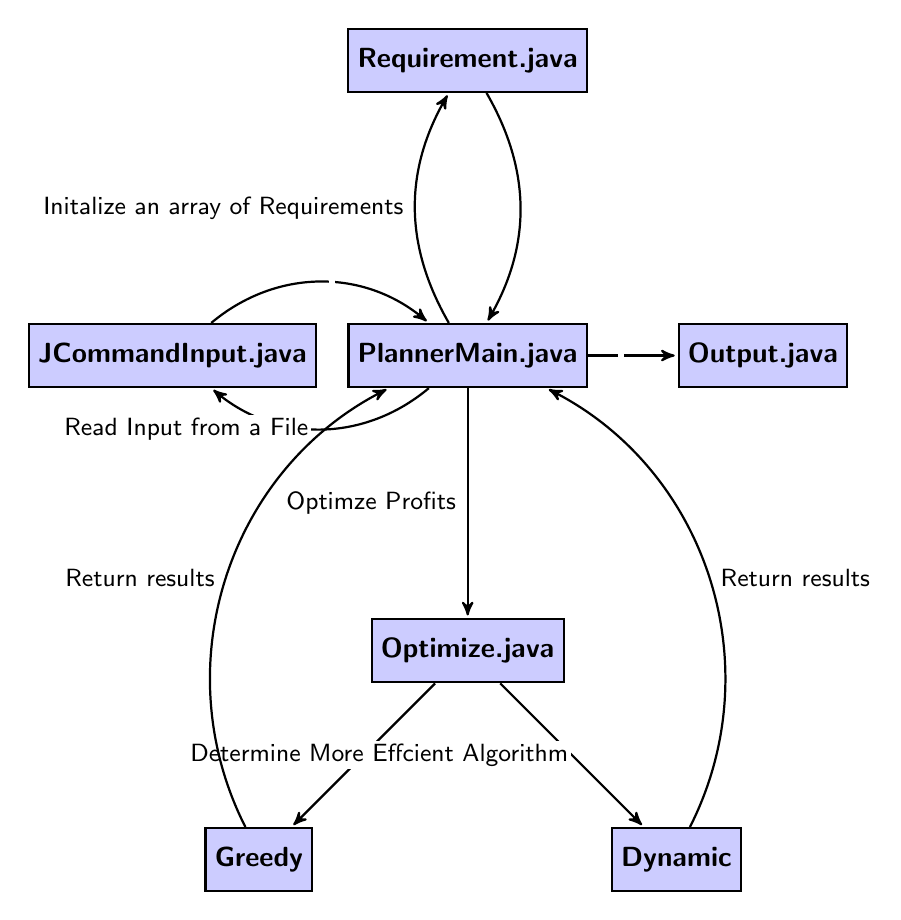
\begin{tikzpicture}[->,>=stealth',shorten >=1pt,auto,node distance=3.75cm,
  thick,main node/.style={rectangle,fill=blue!20,draw,
  font=\sffamily\bfseries,minimum size=8mm}]

  \node[main node] (M) {PlannerMain.java};
  \node[main node] (In) [left of=M] {JCommandInput.java};
  \node[main node] (R) [above of=M] {Requirement.java};
  \node[main node] (O) [below of=M] {Optimize.java};
  \node[main node] (G) [below left of=O] {Greedy};
  \node[main node] (D) [below right of=O] {Dynamic};
  \node[main node] (Out) [right of=M] {Output.java};

  \path[every node/.style={font=\sffamily\small,
  		fill=white,inner sep=1pt}]
    
    %Connects JCommandInput.java to PlannerMain.java%
    (M) edge [bend left=40] node[left=1mm] {Read Input from a File} (In)
    (In) edge [bend left=40] node[right=1mm] {} (M)
    %Connects Requirement.java to PlannerMain.java
    (M) edge [bend left=30] node[left=1mm] {Initalize an array of Requirements} (R)
    (R) edge [bend left=30] node[left=1mm] {} (M)
    %Straight ling from PlannerMain.java to Optimzer.java%
    (M) edge node[left=1mm] {Optimze Profits} (O)
    %Shows decision between greedy and dynamic after Optimzer.java%
    (O) edge [left=40] node[left=1mm] {} (G)
    (O) edge [left=40] node[] {Determine More Effcient Algorithm} (D)
    
    %Shows the return of information from Algortihm choice back to PlannerMain.java
    (G) edge [bend left=45] node[left=1mm] {Return results} (M)
    (D) edge [bend right=45] node[right=1mm] {Return results} (M)
    
    %From PlannerMain.java to Output.java
    (M) edge node[left=1mm] {} (Out);	
	
\end{tikzpicture}
\end{document}\textsl{•}